\section{Data Exploration}

\subsection{Getting the data}
The first challenge was simply downloading and unpacking the files on our Linux systems. Using different GUI tools failed, and in the end, the method that worked was simply concatinating the files into a temporary zip file using \texttt{cat}, and then unzipping the combined file using \texttt{unzip}.\\
\\
Trying to read the data in python proved to be a challenging task, as the .csv file seemed to be corrupted or malformed with rows containing different amounts of columns. After some manual exploration, we found the problem which turned out to be carriage returns. Some article content included \texttt{\textbackslash r}, which was interpreted as "newline", and thus, a new row in the middle of arbitrary news content. A single command '\texttt{sed 's/\textbackslash r/ /g' in.csv > out.csv}' replacing the carriage returns with spaces (to preserve word boundaries) turned out to solve this issue.\\
% \todo{Perhaps missing a section on summary statistics?}

After getting the data into readable CSV file, we decided to load it into a SQL database for easier handling and
exploration.

\subsection{Larger than memory datasets}
Due to the size of our dataset, we had to use different methods for handling our data despite it being larger than
memory. Throughout this report we used 3 different methods: SQL Databases, chunk-wise operations and brute force (acces
to a large enough server). After getting the data into a readable CSV file in the previous step, we decided to load it
into an SQL database for easier handling and exploration. In later sections we will use the other two methods as they
are more appropriate for specific machine learning tasks.


\subsubsection{Summary of the dataset}
Here is main bulletpoints of the data.

\begin{enumerate}
  \item The dataset contains $ 8.528.956 $ articles.
  \item The articles are sorted into the following categories: [bias, clickbait, conspiracy, fake, hate, junksci (junk
    science), political, reliable, rumor, satire, unknown, unreliable]
  \item The number of articles in each category is distributed as seen in figure \ref{fig:combdist}
  \item The dataset contains many articles from just a few publishers, as can be seen in figure \ref{fig:combdist}.
\end{enumerate}

\begin{figure}[htpb]
  \centering
  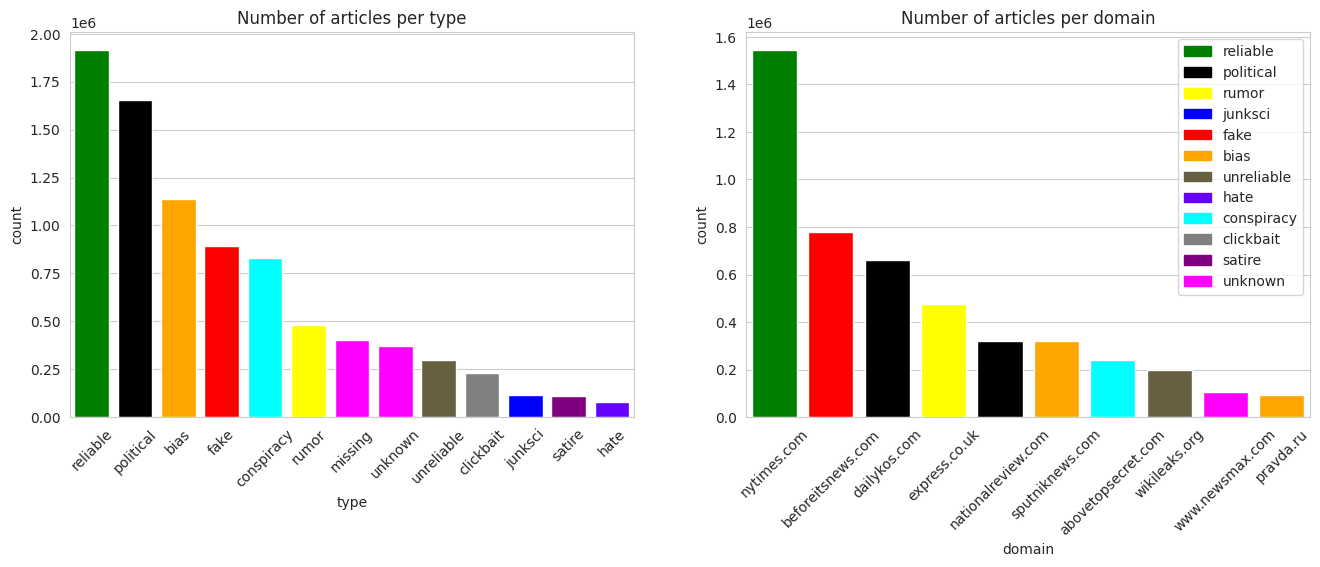
\includegraphics[width=1\textwidth]{combdist}
  \caption{Article type and domain distribution}
  \label{fig:combdist}
\end{figure}
\subsubsection{Vocabulary sizes}
After getting the data into a managable format, we where then able to start properly exploring it. The first thing we
did was to calculate the vocabulary size of the dataset. We did this by first tokenizing the data, and then counting the
unique tokens. We then repeated this process after removing stopwords, and finally after stemming the tokens. The
results are shown in table \ref{tab:vocab_sizes}. As we can see the vocabulary decreases slightly after removing
stopwords, and significantly after stemming. This is expected, since stopwords are a list of (relatively few) very
common words, which is why it doesn't affect the vocabulary size much. However the major decrease after stemming makes
sense, as stemming reduces the number of unique tokens by grouping together words with the same root.


\begin{table}[h]
    \centering
    \begin{tabular}{r| c | c | c| c}
      Data& vocabulary size & vocabulary size (lowered) & \% decrease & \% decrease (lowered)\\
        \hline
      Sample data& 21016 & 18011 & 0\% & 0\% \\
    \hline
      Removed stopwords & 20674 & 17865 & 1.63\% & 0.81\% \\
    \hline
      Stemmed & 12654 & 12703 & 39.8\% & 29.5\%
    \end{tabular}
    \caption{Vocabulary sizes}
    \label{tab:vocab_sizes}
\end{table}

% TODO ADD THESE NUMBERS TO TABLE


\subsubsection{Classifiyng truth per. domain}\label{sec:truth_pr_domain}
One important aspect in the dataset, is how it classifies a news articles into the categories. The creators of the
dataset has chosen to classify the articles per domain, meaning that all the articles from any given domain will be
given the same level of credibility. Ignoring the ethical implications, this meant that we quite quickly realised that
we had to exclude domain from any of our training, as the model would quickly just use the domain only for
classification.
\subsubsection{Duplicated articles}\label{sec:dup_articles}
Another things we realised quite quickly, is that the dataset contains a significant amount of duplicated articles as
seen in table \ref{tab:dupart}.

\begin{table}[htpb]
  \centering
  \caption{Duplicated articles and their domain}
  \label{tab:dupart}
  \begin{tabular}{r | c | c| c}
    domain & type & content & count \\ \hline
    nationalreview.com & political & Plus one article on Google Plus (Thanks to al... & 273388 \\ \hline
    wikileaks.org & unreliable & Tor Tor is an encrypted anonymising network t... & 169259 \\ \hline
    sputniknews.com & bias & Dear readers, we are excited to announce that ... & 102671 \\ \hline
    abovetopsecret.com & conspiracy & It looks like you're using an Ad Blocker. Ple... & 72978 \\ \hline
    investmentwatchblog.com & bias & It only takes a few moments to share an articl... & 35490 \\ \hline
    dailykos.com & political & © Kos Media, LLC Site content may be used for... & 29649 \\ \hline
    sputniknews.com & bias & E-mail: Screen Name: Password: Confirm pass... & 27668 \\ \hline
    lifenews.com & bias & FAIR USE NOTICE. Many of the stories on this s... & 24796 \\ \hline
    express.co.uk & rumor & Express. Home of the Daily and Sunday Express... & 23216 \\ \hline
    nytimes.com & reliable & Opinion >> Should Beach Privatization Be Allowe... & 23035
  \end{tabular}
\end{table}
As we can see, this is due to different popups that the webscraper has encountered as it
was trying to scrape the dataset, such as the $ 169.259 $ articles from Wikileaks all sharing:
\begin{quote}
    \textit{Tor}

    \textit{Tor is an encrypted anonymising network that makes it harder to} [\dots]\\

\end{quote}
These duplicated articles were simply removed before we trained our model.

\subsubsection{Lower dimensionality exploration WIP}
We have made a 2D UMAP representation of the dataset, which is a form of non-linear dimensionality reduction. We've
trained the model unsupervised to get the inherent distribution of the data without any labelling bias.
\begin{figure}[htpb]
  \centering
  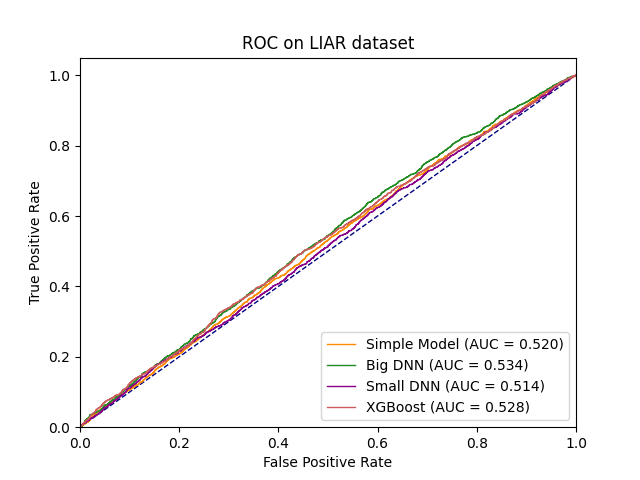
\includegraphics[width=0.8\textwidth]{figures/ROC_LIAR}
  \caption{UMAP representation}
  \label{fig:umap_explore}
\end{figure}

The plot contains a large cluster which contains a rough mix of everything which UMAP couldn't separate as well as some more concentrated cluster of junk science and conspiracy articles. On the boundaries of this cluster, we have some more concentrated clusters that the model was able to separete, this includes reliable, fake. Away from the main cluster, we have a large cluster of almost entirely reliable content the model was easily able to separate from everything else, other clusters far apart include unreliable, rumors and highly invariate hate news and satire (very small concentrated clusters). This serves as our justication for our binary grouping of the dataset since realiable articles are clearly delineated from the rest of the dataset. 



